% Chapter 1

% variables
\newcommand{\pdirone}{chapters/plots/chapter1}

% cross references

\chapter{Why Dark Matter?} % Main chapter title
%\chapter{Introduction} % Main chapter title

\label{chapter1}

Physics is a wonderful thing, I was always mesmerized by its ability to describe what surround us in a powerful and compact way, ultimately using this knowledge for the betterment of the mankind. When I was young, equations were like an ancient magic language to me. I was not able to understand it yet, but I was absolutely impressed by knowing that people that could, were able to control power that for a kid look like beyond any form of comprehension, from making incredibly heavy object flying faster than any bird, or destroying entire city by splitting something invisible for the naked eye. I always dreamed at some point to become part of this exclusive club of magician, and now that I am, I have to say: I got it all wrong! Physics requires a lot of thinking, a lot of reading, a lot of trial and error, in one word? A lot of work! What follows is my attempt to make a lasting contributes to this amazing field. It won't go to history, but I hope it will be important for some students that follow the scientist step, for sure it will be important to me.

So what is this thesis about? Dark Matter, if I had to use one word. One of the most prominent puzzle in all physics. With all our powerful and extremely precise models, we still have to explain more than 96\% of the matter in our universe. That is embarrassing! How could we miss all that? Turns out is not simple at all, when the matter that you are searching for stubbornly refuse to interact with your detectors, but I am sure that eventually physics will prove to be even more stubborn in their measurement, and eventually crack the code. This thesis was an attempt to this, an experiment to produce this elusive matter directly, in the attempt to measure its property. Since my group does not have a noble price in its hand, it must be no mistery that we did not yet succeeded, although this is not excluded for the future. I think the journey of me and the rest of my collegues is nevertheless very instructive, it is the typical story of how an experiment is born and conducted. An "happy ending" is not always expected, and should not be assumed by the scientist that is conducting the experiment, you are just there to observe, not decide. In my opinion, the experiment itself is the "happy ending" that a scientist is seeking, when it is well performed, and that is not depending on the final outcome of it. So with no further wait we can begin our journey, at the discovery of the NA64 experiment and its search of Dark Matter.

In this chapter our story begin, and as every story of science it begins with a mistery: Dark Matter. Why can't see it? Why can't we touch it? Those are not interesting questions, since many well understood phenomena can't be seen or touched. In the end it all boils down to one question: Why our models, that works so amazingly well in so many different situations, fail miserably in other situations apparently completely equivalent? This is what this chapter will be about, understand why we need the concept of dark matter, and justify what phenomena it could explain. Indeed one could think that is rather lazy to explain phenomena just by adding invisible matter in the system. "Just admit that you don't know what is going on!", is something that I heard myself when I try to explain my work to others. That is overall an honest question, an healthy scientific skepticism  about a theory that seems so arbitrary. In Sec.\ref{ch1:sec:dm-evidence} we will explore why we need this concept, and what are the alternatives to it. After that, we will come to realize that Dark Matter is a very simplistic term, that hides an extremely large number of possibilities that can be constructed using the framework of Quantum Field Theory (QFT). Dark Matter candidates are indeed very numerous, potentially even infinite, but we can focus on the most reasonable ones, that do not require extremely complicate model. In agreement with the scientific method, we try to extend our theory minimally, to see if it works, and only after we fail we add more complexity to our new model. In Sec.\ref{ch1:sec:dm-candidates} we will give a small review on these possibilities, trying to be succint but complete. After that, we will introduce the framework of thermal Dark Matter, one of the most successful in describing the observed relic density in our cosmos, that has the indisputable advantage of relating the mass of the Lightest Dark Matter (LDM) candidates with the cross section of annihilation. After these introductions we will finally concentrate ourself to a more specific model, which is one of the main focus of this thesis: the $U'(1)$ model. This model postulates the existence of an additional $U(1)$ symmetry that generates a "Dark Sector" of particles amounting to the invisible matter. The gauge boson of this symmetry, that we will label $\DM$ through this thesis, has been know with the catchy name of Dark Photon, due to playing the equivalent role of the standard model photon in this new symmetry. This model allows also a cross-term that couples the new Dark Photon with its standard counterpart, effectively building a portal between the two sectors. This is excellent news! It means we can produce this type of matter using modern accelerator if such model is true, which allow us to perform a particle physics experiments to probe this model. But why this model should be better than the others? There is not an easy answer to this. From scientific point of view, a model is better than another if it is more powerful in explaining the reality of things. In a framework as complicate as cosmology however, there are countless models that are equivalent in describing reality, which is why so many Dark Matter candidates exist. In a way, it is unavoidable that we share the work and probe all models one by one. However, sometimes a model can solve more than one problem at the same time, which would make them especially attractive for scientist. Originally, the Dark Photon was also an excellent explanation of the measured value of the anomalous muon magnetic moment, that to date deviates substantially (by 3.5 standard deviation) from the prediction of QED. We now know that such explanation is ruled out, since NA64 together with other experiments excluded it. Another interesting phenomena that could be explained is the so called $\DMX$-anomaly, originally known with the name of $^8$Be-anomaly. This name refers to an anomaly detected in the nuclear decay spectrum of Beryllium that would be justified by the existence of a particle not present in the standard model. This anomaly was later confirmed in the $^4$He atom as well, which makes it a very interesting phenomena to study. In Sec.\ref{ch1:sec:dm-u1model-motivations-x17} a review of this phenomena will be given. To avoid confusion, we point out here that the $\DMX$, which is the name given to the particle advocated to explain the observed anomaly, is not by definition a Dark Photon, since it posses some properties that are not present in a more vanilla model. However, its characteristic are similar enough to be probed by the NA64 experiment, as it will be clear from this thesis.

This chapter is meant to just answer the question: what are we searching for? This is the beginning of every scientific experiment, but arguably the easiest part! Building an experiment to produce the Dark Photon is the next step, which will be covered in chapter \ref{chapter2}. Turn a photon in a Dark Photon using this portal is however meaningless if we can't prove that we did it! A robust analysis method of the data collected need to be performed for this purpose, this is what we will explore in chapter \ref{chapter3} step by step, from the method to the selection criteria. In chapter $\ref{chapter4}$ we will than provide what most scientist are here for, the results! No Dark Matter has been found yet, but the data acquired allow us to exclude some specific models from being allowed credible explanation of reality. To reiterate an example already used: we now know thanks to this data, that the anomalous magnetic moment of the muon cannot be explained exclusively bu the $U'(1)$. The NA64 experiment is however far from over! The break given by the LHC long shutdown (and unfortunately by the recent rise of Covid-19 as well) allowed us to stop for a second a look for ways to improve our setup for the upcoming challenges of 2021! The knowledge we gained for the background and the experimental condition are used to design the new version of the setup to acquire a larger number of particles and thus probe a larger number of models. In chapter \ref{chapter5} we will review all these changes, in particular the new setup for the visible mode of 2021, that was the last project of my PhD, and that will use to hopefully find (or else exclude) the $\DMX$.

With no further wait, let's embark ourselves in this journey!

%----------------------------------------------------------------------------------------

\section{Evidence for Dark Matter}
\label{ch1:sec:dm-evidence}

The story of Dark Matter and the birth of this term is interesting on its own, and a good example of "unequivocal accumulated evidence" in science, but in a way is even more than that \cite{hooper, deSwart:2017heh}. The terms was first used in 1937 by astronomer Fritz Zwicky\footnote{Some weaker claim of a discrepancy were done even before by Knut Lundmark in 1930.} to justify the velocity dispersion in Coma cluster galaxies, which were deviated significantly from what predicted by simply asserting the mass from the visible matter. This hypothesis was discussed more seriously on in 1950, when astronomical surveys confirmed this results with high precision. This sparked an heated debate in the scientific community, and understandably many solutions to this problem did not include additional unknown matter, but rather modification of gravity or more sophisticated arguments based on dynamical equilibrium of such galaxies. In 1970 with the rising of radio astronomy the rotation curved of galaxies are studied in detail, and two studies performed by Kenneth Freeman and Vera Rubin separately confirm that the velocity or rotation of objects in a galaxy becomes flat at sufficient distance from its center. The idea becomes very influential to the cosmological community thanks to two very influential paper in 1974 by Einasto and Ostriker, that clearly states that the mass of galaxies has been underestimated by a factor 10 until then \cite{EINASTO1974,1974ApJ...193L...1O}. This was further strengthen by the end of the decade by very similar analysis, and well summarized in this review \cite{annurev.aa.17.090179.001031}. The existence of Dark Matter becomes more and more accepted in the years to come, both alternative theory also arise to explain observation without the need of additional matter. Pheraps the most famous today remains the MOND theory, theorized as a weak-field approximation of some more general theory of gravity yet to be discovered. Despite some early success, this theory has always proven to be challenging to merge in the general relativity framework, and is insufficient to justify some specific phenomena like the famous "bullet cluster", that is on the other hand very well explain by Dark Matter \cite{Clowe_2006}.

So what is the current situation of Dark Matter? Today the theory is well accepted in the scientific community, although some debate and alternative theory are still present, the existence of Dark Matter is the leading paradigm to explain all discrepancy observed \cite{hooper}. Outside from the compelling arguments listed above, advances in the field of cosmology and measurements technique have provided many other evidence that aid Dark Matter existence. For example gravitational lensing, in particular in the context of weak lensing, was used to characterize the mean distribution of Dark Matter and match it to the one predicted by large scale structure measurements \cite{weak-lensing}. The measurements of temperature anisotropies of the Cosmological Microwave Background (CMB) present structures compatible with Dark Matter, and well fitted in the $\Lambda$CDM model that we will introduce in Sec.\ref{ch1:sec:dm-thermal} \cite{Ade:2015xua}. On the top of this, many other arguments, including structure formation \cite{Navarro:1995iw}, baryon acoustic oscillation \cite{bao}, and Red-shift distortions \cite{Peacock2001} have proven consistently in agreement with Dark Matter existence and in particular with the $\Lambda$CDM model.

So let us assume like the majority of scientific community that Dark Matter indeed exist, what is it the exact nature? Can we point down some characteristic and a space of parameter that defines it exactly? Those are the questions that will be answered in the next section.

\section{Dark Matter candidates}
\label{ch1:sec:dm-candidates}

The first to ask ourselves is what kind of property Dark Matter should have to satisfy the experimental constraint given by cosmology. Following the excellent book of Stefano Profumo \cite{Profumo:2019ujg}, we can define the following properties:

\begin{itemize}
\item \textit{Dark}: Trivially enough, Dark Matter should not emit light, but a tiny charge is still compatible with data, which justifies models with "milli-charges" particles. What is effectively constraint is the ratio of charge to some power of the mass.
\item \textit{Collisionless}: Dark Matter self-interaction to mass ratio is constraint by observation of cluster mergers and the ellipticity of galactic halos. The cross-section itself is not however necessarly small, assuming a mass similar to the one of a proton, indeed the constraint amount to a cross section in the order of barn, very similar to the one observed for strong interaction.
\item \textit{Classical}: Dark Matter is observed to be confined on the galactic scales of a few kpc in dwarf galaxies. Hence, their de Broglie length must be smaller than that to have a coherent Dark Matter halo. This argument is typically used to put a lower limit on the DM mass. If the Dark Matter candidates is a fermion, constraints are stronger as Pauli blocking limits the density to at most the phase space density to $f=gh^{-3}$ where g are the number of internal degrees of freedom.
\item \textit{Fluid}: For macroscopic DM, with mass much larger than the solar mass $M_{\odot}$, tidal disruption is expected to break the stability  in global cluster. This limit is typically placed around $10^6 M_{\odot}$.
\end{itemize}

In summary, while the cosmological and Galactic Dark Matter density is known to a good degree, very weak constraint exist on the interaction strength and the exact mass of Dark Matter. The huge mass scale that spans over the possible region is excellently depicted in Fig.\ref{fig:dm-mass-range}, where we see several possible DM candidates in relation with their possible mass and search technique to probe them. In red we can also see a few experimental anomalies

\begin{figure}[bht!]
  \centering
  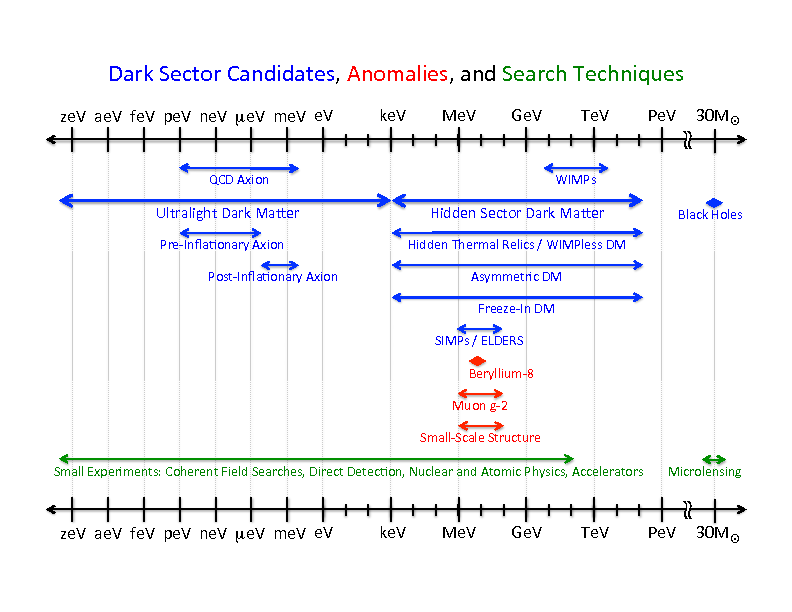
\includegraphics[scale=0.5]{\pdirone/DM_summary.png}
  \caption[Mass range for Dark Matter]{Mass range for Dark Matter and mediator particle candidates, experimental anomalies, and search techniques \cite{battaglieri2017cosmic}.}
  \label{fig:dm-mass-range}
\end{figure}

\subsection{Thermal Dark Matter}
\label{ch1:sec:dm-thermal}

\subsection{Dark Matter in colliders}
\label{ch1:sec:dm-colliders}

Dark sectors are very interesting candidates to explain the origin of Dark Matter (see e.g. \cite{mb} for a recent review), whose presence has 
so far been inferred only through its gravitational interaction from cosmological observations \cite{hooper}. 
If, in addition to gravity, a new force between the dark sector and visible matter exists \cite{prw, pospelov} this can be tested in laboratory experiments. A possibility is that this new force is carried by a vector boson $A'$, called dark photon.
Stringent limits on the coupling strength $\epsilon$ and mass $m_{A'}$ of such dark photons, excluding the parameter space region favored by the anomalous magnetic moment of the muon, the so called $(g-2)_{\mu}$ anomaly, have already been placed by beam dump \cite{jdb, charm, rio, e137, konaka, bross, dav,  ath, nomad, e787, essig1, blum,sg1, blum1, sarah1}, fixed target \cite{apex,merkel,merkel1}, collider \cite{babar, curt, babar1}, rare particle decay searches \cite{sindrum, kloe, sg2, kloe2, wasa, hades, phenix, e949, na48, pol, kloe3} and the new determination of the fine structure constant $\alpha$ combined with the measurement of $(g-2)_e$ \cite{Parker191,PhysRevLett.100.120801}.

\section{The U'(1) model}
\label{ch1:sec:dm-u1model}

\begin{equation}
  \label{eq:dm-rate}
  N_{\DM} \sim N_{EOT} \times C' \epsilon^2 \frac{m_e^2}{m^2_{\DM}}
\end{equation}

\subsection{Decay modes}
\label{ch1:sec:dm-decay}

\subsubsection{Invisible decay mode}
\label{ch1:sec:dm-decay-invis}

\subsubsection{Visible decay mode}
\label{ch1:sec:dm-decay-vis}


\begin{eqnarray}
  L_{\DM} = 28.3 ~{\rm mm}  \Bigl[\frac{E_{\DM}}{100~ {\rm GeV}}\Bigr] 
  \Bigl[\frac{17~ {\rm MeV}}{m_{\DM}}\Bigr]^2 \Bigl[\frac{10^{-3}}{\epsilon}\Bigr]^2
  \label{eq:dm-decay-length}
\end{eqnarray}

\subsection{The X17 anomaly}
\label{ch1:sec:dm-u1model-motivations-x17}

A great boost to search for the new light boson weakly coupled to Standard Model particles was triggered by the recent observation of a $\sim$7$\sigma$ excess of events in the angular distribution of $\pair$ pairs produced in the nuclear transitions of the excited $^8$Be$^*$ nuclei to its ground state via internal $\ee$ pair creation \cite{Krasznahorkay:2015iga}. The latest results of the ATOMKI group report a similar excess at approximately the same invariant mass in the nuclear transitions of another nucleus, $^4$He \cite{Krasznahorkay:2019lyl}.

It was put forward  \cite{Feng:2016jff,PhysRevD.95.035017}, that this anomaly can be interpreted as the emission of a protophobic gauge boson $\DM$ decaying into $\pair$ pairs. To be consistent with the existing constraints, the $\DM$ boson should have a non-universal coupling to quarks and a coupling strength with electrons in the range of $2\times 10^{-4} \lesssim \epsilon_e \lesssim 1.4\times 10^{-3}$ which translates to a lifetime of the order of $10^{-14}\lesssim \tau_X \lesssim 10^{-12}$~s. Remarkably, this model also explains within experimental uncertainty the new result obtained with the $^4$He nucleus, providing both kinematical and dynamical evidence to support this interpretation \cite{Feng:2020mbt}. This model will be used as benchmark for the NA64 current results and to cast the sensitivity of the new setup described in this article. However, other solutions of the $\DM$ anomaly were proposed, see for example \cite{Nam:2019osu, Seto:2016pks}.

Interestingly, such a new boson with a relatively large coupling to charged leptons could also resolve the tension between measured and predicted values of the $(g - 2)_{\mu}$. In addition to vector and axial-vector explanation of the $\DM$ anomaly, one can consider scenarios involving hidden pseudo-scalar boson \cite{Ellwanger:2016wfe}. Corresponding pseudo-scalar couplings to electrons satisfy existing experimental constraints \cite{Andreas:2010ms,Adler:2004hp}. An analysis to probe such pseudo-scalar states at NA64 \cite{Kirpichnikov:2020tcf} would require a proper Monte-Carlo simulation of the spectra and flux of light pseudo-scalar boson produced in the target by electrons.
Another interesting result comes from the new measurement of $\alpha$ performed by Parker et al. \cite{Parker191} which combined with the $(g-2)_e$ measurements result in a 2.4$\sigma$ deviation from the QED predictions \cite{PhysRevLett.100.120801}. Should this tension be confirmed, the two constraints coming from the NA64 results and $(g - 2)_e$ would exclude the vector and axial vector couplings explanation of $\DM$. On the other hand, models with nonzero V$\pm$A coupling constant with the electron would explain both electron and muon $(g - 2)$ anomalies \cite{Krasnikov:2019dgh}. In these models, the $\DM$ could have a coupling of $6.8\cdot 10^{-4} \lesssim \epsilon \lesssim 9.6 \cdot 10^{-4}$ which leaves an interesting region of the parameter space to be explored.
These models motivated the study of the phenomenological aspects of such a light vector boson weakly coupled to quarks and leptons (see, e.g., Refs.~\cite{fayet1, fayet2, fayet3, fayet4,jk, cheng, Zhang:2017zap, ia, liang, bart}) 
and new experimental searches (see e.g., Refs.~\cite{mb, nardi}).

Recently, the NA64 collaboration has reported new results that excluded the $\DM$ boson  with the coupling strength  to electrons in the range $1.2 \times 10^{-4} < \epsilon_e < 6.8 \times 10^{-4}$ \cite{Banerjee:2018vgk,Banerjee:2019hmi}, by using the calorimeter technique proposed in \cite{Gninenko:2013rka,Andreas:2013lya}. In this work, the main challenges to search for large coupling $\epsilon \sim 10^{-3}$ of $\DM$ will be outlined and an upgrade of the setup to overcome them is described. First, in Sec.\ref{ch3:sec:vis-mode-veto} an overview on the calorimeter method \cite{Gninenko:2013rka,Andreas:2013lya,Banerjee:2019hmi} is presented and the main limitations of the current setup are outlined. In Sec.\ref{ch3:sec:vis-mode-tracking}, a new analysis method that exploits the trackers is presented. This analysis highlights the importance of an efficient tracking procedure for the $\DM$ search. The increase in sensitivity is however negligible due to the intrinsic limitations of the setup.

%%% Local Variables:
%%% mode: latex
%%% TeX-master: "../PhDthesis"
%%% End:
